\documentclass[conference,a4paper]{IEEEtran}
\pdfminorversion=6
\usepackage[utf8]{inputenc}
\usepackage[T1]{fontenc}
\usepackage{amsmath}
\usepackage{amssymb}
\usepackage{graphicx}
\usepackage{booktabs}
\usepackage{array}
\usepackage{tikz}
\usepackage{pgfplots}
\pgfplotsset{compat=1.17}
\usetikzlibrary{arrows.meta, positioning, shapes.geometric, calc}

\begin{document}

\title{CropState-Vision: A Reliability-Oriented Evaluation of Six-Stage Rice Growth Classification and Confidence-Aware Stage-Gated Retrieval}

\author{
\IEEEauthorblockN{Nguyen Quoc Minh Phan, Bao Nhi Le, Khanh Nhi Le}
\IEEEauthorblockA{FPT University -- Da Nang Campus\\ Da Nang, Viet Nam\\
\{minhpnq1807, lebaonhi0805, nhilekhanh29\}@gmail.com}
\and
\IEEEauthorblockN{Thi To Tam Tran\IEEEauthorrefmark{1}}
\IEEEauthorblockA{FPT University - Da Nang Campus\\ Da Nang, Viet Nam\\
tamttt14@fe.edu.vn}
}

\maketitle

\begin{abstract}
CropState-Vision studies six morphology-derived, BBCH-inspired rice pseudo-stages and uncertainty-aware evidence retrieval. A three-seed fixed-split ResNet-18 evaluation on 2{,}900 RiceSEG-derived crops reaches 0.800 mean accuracy against weak labels, not expert-confirmed phenology. We correct the retrieval protocol to use English BM25 queries for 173 English-language IRRI chunks, and evaluate 420 metadata-labeled scenarios from 199 crops belonging to 63 original photographs. Adaptive gating yields nDCG@5 of 0.545 versus 0.343 for query expansion and metadata-defined SIRR@5 of 0.127 versus 0.301. Hard filtering has SIRR@5 of 0.011 but does not return five documents in 10\% of scenarios. Validation selects fixed-soft $\beta=0.35$, which reaches nDCG@5 0.612 / SIRR@5 0.101, and a top-1-belief variant reaches 0.617 / 0.098; both outperform combined-confidence adaptive gating on these metadata metrics. Paired uncertainty estimates resample the 63 original parent photographs, with Holm-adjusted tests. Results establish an internally consistent evaluation of stage-conditioned retrieval; neither expert-judged BBCH accuracy nor agronomic usefulness or safety is demonstrated.

\end{abstract}

\begin{IEEEkeywords}
rice growth stage, BBCH, image classification, ordinal loss, calibration, selective prediction, stage-aware retrieval, data leakage
\end{IEEEkeywords}

\section{Introduction}

Rice management recommendations depend on growth stage: irrigation, nutrient scheduling, disease surveillance and harvest preparation must follow plant development rather than the calendar. Crop-stage recognition from field images is challenging near phenological transitions and under changes in lighting, viewpoint and plant density. Overconfident mistakes can propagate into retrieval if a top-1 stage prediction is treated as certain.

CropState-Vision retains a six-stage probability distribution and uses it to adjust metadata-driven evidence reranking. The aim is a reproducible, reliability-oriented \emph{evaluation}, not a novel vision backbone, a new retrieval model, or an autonomous agronomic advisor.

We address three linked questions: (RQ1) What can be concluded about six-stage visual classification and selective prediction on a fixed, near-duplicate-audited split? (RQ2) What ranking versus stage-incompatibility trade-offs arise for hard, fixed-soft and confidence-adaptive retrieval? (RQ3) Which evidence limitations constrain these findings? Our contributions are:
\begin{enumerate}
    \item A group-aware aHash duplicate audit and three-seed ResNet-18 comparison, with ordinal, class-imbalance and calibration reporting on \emph{morphology-derived} reference labels.
    \item An English-query, metadata-defined retrieval benchmark of 420 topic scenarios, using 63 original-parent-photo clusters for paired bootstrap and sign-flip inference.
    \item Validation-only comparison of tuned fixed-soft weights, full-belief, top-1, entropy and margin variants, including unfavorable results for the original adaptive formula and underfilled hard-filter outputs.
    \item Explicit boundaries: weak phenology labels, small rare-stage classes, a single dataset split, and relevance scores sharing stage metadata with the reranker.
\end{enumerate}

\section{Related Work}

The BBCH scale gives standardized numerical descriptions of plant development \cite{meier2001bbch}. We group fine-grained rice codes into six macro-stages as a classification convenience, not a BBCH replacement. Machine learning has been applied to rice development from field imagery \cite{tan2022machine}; RiceRes2Net detects panicles and recognizes three reproductive sub-stages \cite{tan2023ricepanicle}, and a lighter YOLO version ships as a smartphone app \cite{zheng2025android}. Both target seedling- or panicle-level sub-stages, whereas CropState-Vision classifies whole images across the vegetative-to-ripening cycle. A random split can overstate field generalization if acquisition cues leak across train/test \cite{kapoor2023leakage}.

ResNet is the pretrained backbone used here \cite{he2016deep}; EfficientNet and Vision Transformers exist but were not evaluated, since the focus is training objective, not architecture search. Temperature scaling checks calibration \cite{guo2017calibration}, and selective classification lets a model abstain on uncertain cases \cite{geifman2017selective}. Predictive uncertainty is known to degrade under distribution shift \cite{ovadia2019trust}, and the aleatoric/epistemic distinction \cite{hullermeier2021aleatoric} motivates treating confidence as a routing signal rather than a correctness guarantee, the stance taken throughout this paper. Focal loss \cite{lin2017focal} is a usual response to class imbalance. The six stages are ordered, not nominal, motivating a distance-aware objective and MASD alongside accuracy \cite{gutierrez2016ordinal}. Statistically, we use bootstrap intervals, Holm correction, and McNemar's test \cite{mcnemar1947note}.

Retrieval-augmented generation grounds language-model output in external evidence \cite{lewis2020rag}: BM25 for lexical matching \cite{robertson2009bm25}, dense retrieval for semantic similarity \cite{karpukhin2020dpr}, fused by Reciprocal Rank Fusion \cite{cormack2009rrf}. CropState-Vision follows this recipe with a sentence-transformer retriever \cite{reimers2019sbert}, adding confidence-aware stage re-ranking. Against the closest rice-stage studies -- \cite{tan2022machine,tan2023ricepanicle,zheng2025android}, which cover only 3 seedling or panicle-level sub-stages and report neither calibration nor significance testing -- CropState-Vision covers all 6 macro-stages and reports ECE/Brier, MASD, and bootstrap/McNemar testing.

\section{Task Formulation}

\subsection{Six Rice Macro-Stages and Stage Belief}

Let $\Phi = \langle \phi_1,\dots,\phi_6 \rangle$ be the ordered stage set in Table~\ref{tab:stages}. For image $I$, model $f_\theta$ produces logits $o = f_\theta(I)$ and the stage distribution $p(\phi_i \mid I) = \mathrm{softmax}(o/T)_i$, with $T>0$ from validation logits when temperature scaling applies. The top-1 prediction is $\hat{\phi} = \arg\max_i p(\phi_i \mid I)$, but we retain the full belief $B = p(\cdot \mid I)$, summarized by normalized entropy $\Gamma = 1 - H(B)/\log 6$ and top-two margin $M = B_{(1)} - B_{(2)}$, combined as
\begin{equation}
p(\phi_i \mid I) = \mathrm{softmax}(o/T)_i, \quad
\kappa = \eta \Gamma + (1-\eta) M,
\label{eq:softmax}
\end{equation}
with $0 \le \eta \le 1$. Here $\kappa$ is a routing signal, not proof the predicted stage is correct.

\begin{table}[t]
\centering
\caption{Rice macro-stages used in the study.}
\label{tab:stages}
\footnotesize
\begin{tabular}{lcl}
\toprule
\textbf{Group} & \textbf{BBCH} & \textbf{Label} \\
\midrule
Germination/leaf development & 00--19 & Establishment \\
Tillering & 20--29 & Tillering \\
Stem elongation/booting & 30--49 & Stem/booting \\
Heading and flowering & 50--69 & Reproductive \\
Grain development & 70--79 & Grain filling \\
Ripening & 80--89 & Ripening \\
\bottomrule
\end{tabular}
\end{table}

\subsection{Confidence-Aware Stage-Gated Retrieval}

Each chunk $x$ carries stage-compatibility $C(x,\phi_i) \in [0,1]$ (1 = direct, intermediate = adjacent, 0 = incompatible). BM25 and dense retrieval give candidate lists fused by RRF and normalized to $S_{\mathrm{base}}(x)$. Expected compatibility, the confidence-scaled stage weight, and the final score are
\begin{equation}
\begin{aligned}
S_{\mathrm{stage}}(x,B) &= \sum_{i=1}^{6} B(\phi_i)\, C(x,\phi_i), \\
\beta &= \beta_{\min} + (\beta_{\max}-\beta_{\min})\,\kappa, \\
S(x) &= (1-\beta)\, S_{\mathrm{base}}(x) + \beta\, S_{\mathrm{stage}}(x,B).
\end{aligned}
\label{eq:score}
\end{equation}
$\beta$ is deliberately linear in $\kappa$ rather than a sigmoid or learned function: with only three seeds and 420 evaluation scenarios there is not enough held-out data to fit a nonlinear mapping without overfitting the operating point, and a linear rule keeps the confidence-to-weight relationship auditable. Unlike top-1 hard filtering, $S(x)$ does not exclude a chunk solely for being incompatible with the most probable stage. Metadata-defined stage incompatibility (not real-world agronomic safety) is measured by
\begin{equation}
\mathrm{SIRR@}k = \tfrac{1}{k}\sum_{x \in \mathrm{TopK}} \mathbb{I}[C(x,\phi^*)=0],
\label{eq:sirr}
\end{equation}
where $\phi^*$ is the morphology-derived reference pseudo-stage; the denominator $k$ is unchanged if fewer than $k$ results are returned.

\section{Materials and Methods}

\subsection{Benchmark Construction and Near-Duplicate Audit}

RiceSEG supplies segmentation masks rather than expert-assigned BBCH stages \cite{zhou2025riceseg}. We use 2{,}900 eligible RGB/mask crops from the 3{,}078 annotated source images. Six BBCH-inspired pseudo-stage labels are derived from segmentation statistics rather than direct plant observations: a panicle fraction cutoff of 0.02 separates panicle-bearing crops; senescence fractions of 0.05 and 0.20 distinguish reproductive, grain-filling and ripening categories. For crops without emerged panicles, canopy-cover fractions of 0.31 and 0.51 distinguish establishment, tillering and stem/booting. These are dataset-specific heuristics, not expert-verified stages.

The fixed split contains 2{,}400 training, 237 validation and 263 test crops, shared by training seeds 42, 7 and 123. Test support is uneven: establishment 54, tillering 88, stem/booting 64, reproductive 24, grain filling 10, ripening 23. The aHash (grayscale 8$\times$8) Hamming audit reports 661 near-duplicate edges at distance $\leq10$ and zero cross-split matches at that threshold (Table~\ref{tab:phash}). The split was grouped by detected near-duplicates; zero audited crossings therefore cannot establish independence across fields, seasons or devices.

\begin{table}[t]
\centering
\caption{Near-duplicate audit over the 2,900-image benchmark.}
\label{tab:phash}
\footnotesize
\begin{tabular}{ccccc}
\toprule
\textbf{Hamming} & \textbf{Near-dup.} & \textbf{Multi-img.} & \textbf{Straddling} & \textbf{Cross-split} \\
\textbf{thresh.} & \textbf{edges} & \textbf{clusters} & \textbf{clusters} & \textbf{pairs} \\
\midrule
10 & 661   & 122 & 0  & 0 \\
12 & 2{,}173 & 131 & 32 & 197 \\
14 & 6{,}712 & 68  & 21 & 999 \\
\bottomrule
\end{tabular}
\end{table}

\subsection{Vision Models and Training Objectives}

The model is an ImageNet-pretrained ResNet-18 (224-pixel input, batch 32, at most 30 epochs, AdamW; head/backbone learning rates $3\times10^{-4}/3\times10^{-5}$; frozen backbone for the first three epochs). All objectives use one fixed split and three training seeds; the checked-in configuration uses class-weighted losses but disables balanced sampling. We compare cross-entropy, an ordinal-aware loss on indices $0,\ldots,5$,
\begin{equation}
L_{\mathrm{ord}}=L_{\mathrm{CE}}+0.5\bigl(\mathbb{E}[y]-y^*\bigr)^2,
\label{eq:ordinal}
\end{equation}
and a weighted focal variant ($\gamma=2$). Its implementation applies $\exp(-L_{\mathrm{CE,weighted}})$ in the modulation factor and is not the standard unweighted focal expression \cite{lin2017focal}. Reported vision metrics are historical fixed-split results; the corrected retrieval experiment does not retrain these vision checkpoints.

\subsection{Retrieval Configuration and Baselines}

The controlled test uses 173 non-restricted English-language IRRI knowledge chunks \cite{irri_knowledge_bank}. BM25 queries are now in \emph{English}, matching the corpus, while multilingual MiniLM-L12-v2 dense embeddings use a verified FP32 ONNX export (128-token cap, masked mean pooling, L2 normalization). We fuse lexical/dense lists with RRF ($k_0=60$, depth 50), use topic-exact candidates and set source-authority weight to zero. The earlier Vietnamese lexical queries gave zero BM25 token overlap and their numeric results are superseded.

A scenario is eligible when a stage/topic pairing has at least three relevant and three incompatible chunks, with metadata relevance defined at compatibility $\geq0.5$. Thus 420 scenarios arise from 199 of 263 test crops, nested in 63 original photographs. Stages and judgments use metadata also consumed by the reranker; they measure internal consistency, \emph{not} independent advice usefulness. Combined adaptive confidence uses entropy concentration (weight 0.6) and top-two margin (0.4), with $\beta_{\min}=0.05$ and $\beta_{\max}=0.35$; fixed B3 has untuned $\beta=0.20$. The reference-stage oracle uses the weak reference pseudo-stage, not an ideal relevance ranking. Table~\ref{tab:methods} defines the alternatives.

\begin{table}[t]
\centering
\caption{Retrieval methods compared.}
\label{tab:methods}
\footnotesize
\begin{tabular}{cp{0.36\textwidth}}
\toprule
\textbf{ID} & \textbf{Description} \\
\midrule
B0 & Ungated BM25+dense retrieval, normalized RRF. \\
B1 & Query expansion: append top-1 predicted stage. \\
B2 & Hard filtering: remove zero-compatibility chunks. \\
B3 & Soft re-ranking, untuned fixed $\beta = 0.20$. \\
P  & Combined-confidence, full-belief adaptive re-ranking. \\
\bottomrule
\end{tabular}
\end{table}

\subsection{Metrics and Statistical Analysis}

Vision metrics include accuracy, macro-F1, ECE, Brier score, Mean Absolute Stage Distance (MASD) and per-class recall against weak pseudo-stage labels. Selective risk is one minus accuracy over retained weak-label test crops. We compute full risk--coverage curves at all 263 sorted top-$k$ prefixes. The exact full-coverage AURC is the mean prefix risk $\frac{1}{263}\sum_{k=1}^{263}R(k)$, rather than a trapezoid over sparse manually chosen thresholds. Retrieval metrics are P@5, R@5, nDCG@5 \cite{jarvelin2002ndcg} and metadata-SIRR@5. Unlike crop-wise resampling, the paired bootstrap and sign-flip tests cluster all topics/crops belonging to the same \emph{original parent photograph} (63 groups), with 5{,}000 resamples and Holm adjustment over 12 pre-specified method--metric comparisons \cite{holm1979sequential}. Incomplete Top-5 returns are measured separately because SIRR@5 divides by five even when fewer chunks are returned.

\section{Results}

\subsection{Stage Classification (RQ1)}

All three objectives clear the majority reference by a wide margin (Table~\ref{tab:vision-results}); differences fall within seed-to-seed noise. Ordinal edges ahead slightly on average, CE keeps the lowest ECE, but one run can flip the ranking (seed 42 alone: ordinal 0.814, CE 0.795).

\begin{table}[t]
\centering
\caption{ResNet-18 results on the 2,400/237/263 split (mean $\pm$ SD over 3 seeds).}
\label{tab:vision-results}
\scriptsize
\setlength{\tabcolsep}{2.5pt}
\begin{tabular}{lccccc}
\toprule
\textbf{Model} & \textbf{Acc.} & \textbf{F1} & \textbf{MASD}$\downarrow$ & \textbf{ECE}$\downarrow$ & \textbf{Rep.rec.} \\
\midrule
Majority   & 0.335 & 0.084 & 1.10 & n/a & 0.000 \\
CE           & $0.800{\pm}.007$   & $0.794{\pm}.019$   & $0.238{\pm}.013$   & $0.062{\pm}.014$   & $0.903{\pm}.052$ \\
Ordinal      & $0.801{\pm}.013$   & $0.796{\pm}.018$   & $0.233{\pm}.013$   & $0.064{\pm}.002$   & $0.917{\pm}.000$ \\
Focal        & $0.767{\pm}.016$   & $0.757{\pm}.014$   & $0.271{\pm}.010$   & $0.179{\pm}.027$   & $0.875{\pm}.059$ \\
\bottomrule
\end{tabular}
\end{table}

The ordinal objective yields identical reproductive recall of 0.917 across seeds on the \emph{same 24 test crops}, compared with CE standard deviation 0.052. This is conditional training variability, not evidence of general stability across independent fields or data splits. Grain filling has only ten test crops; focal yields lower accuracy and worse calibration \emph{under its implemented weighted formulation}. Seed-42 CE versus ordinal comparisons show no statistically resolved accuracy difference ($p=0.40$) or MASD difference ($p=0.21$), and reproductive McNemar testing is underpowered ($b=2,c=0,p=0.50$).

\subsection{Selective Prediction}

On seed-42 CE logits, validation-set temperature scaling gives $T=0.875$. The full-test weak-label risk is 0.2053. A confidence threshold of 0.524541, chosen exclusively on 237 validation logits to target approximately 70\% coverage, retains 189/263 test crops (coverage 0.7186) at weak-label selective risk 0.1217. Using all 263 ranked test prefixes, the exact AURC is 0.1042 for combined entropy/margin confidence and 0.1036 for max-softmax. The previous AURC 0.126 was a trapezoidal estimate over 14 sparse confidence thresholds, normalized by the observed coverage span (0.285--1.0), rather than all nonempty prefixes; it is superseded by the full-coverage AURC. The historical coverage 0.5399/risk 0.0986 point used a \emph{max-softmax threshold of 0.8}, not the combined-confidence score; Fig.~\ref{fig:risk-coverage} therefore shows two separately labeled curves. The 189/263 retained validation-selected point belongs to the combined-confidence curve and was not fitted to test labels. Neither curve establishes expert-confirmed BBCH correctness.

\begin{figure}[t]
\centering
\resizebox{0.99\linewidth}{!}{% Empirical, test-only FULL risk--coverage profiles (N=263).
% Data are generated by scripts/experiments/export_risk_coverage.py from
% validation-calibrated logits, not interpolated or hand-selected coordinates.
% Main blue line uses combined entropy/margin confidence (validation-selected).
% Gray dashed line uses max-softmax (the historical post-hoc example).
% These are DIFFERENT confidence functions: do not join their markers.
\begin{tikzpicture}
\begin{axis}[
  width=8.2cm,height=5.7cm,
  xlabel={Test coverage},
  ylabel={Weak-label selective risk},
  xmin=0,xmax=1.02,ymin=0,ymax=0.27,
  xtick={0,0.25,0.5,0.75,1},
  ytick={0,0.05,0.10,0.15,0.20,0.25},
  tick label style={font=\scriptsize},
  scaled y ticks=false,
  yticklabel style={/pgf/number format/fixed, /pgf/number format/precision=2},
  label style={font=\scriptsize},
  grid=major,grid style={line width=0.1pt,draw=black!15},
  legend style={font=\tiny,at={(0.5,-0.20)},anchor=north,
                legend columns=2,draw=none,fill=none,
                /tikz/every even column/.append style={column sep=0.3cm}},
  legend cell align=left,
  clip=true,
]
\addplot[very thick,blue!80!black,no marks]
  table[x=coverage,y=risk,col sep=comma]
  {images/risk_coverage_points.csv};
\addlegendentry{Combined confidence ($\kappa$)}
\addplot[thick,densely dashed,gray!75!black,no marks]
  table[x=coverage,y=risk,col sep=comma]
  {images/risk_coverage_maxsoftmax.csv};
\addlegendentry{Max-softmax}
\addplot[only marks,mark=star,mark size=3.2pt,red!75!black]
  coordinates {(0.7186311787,0.1216931217)};
\addlegendentry{Validation-selected $\tau$}
\addplot[only marks,mark=triangle*,mark size=2.5pt,black]
  coordinates {(1.0,0.2053231939)};
\addlegendentry{Full coverage}
\addplot[only marks,mark=o,mark size=2.7pt,gray!75!black]
  coordinates {(0.5399239544,0.0985915493)};
\addlegendentry{Historical $\max p$ point}
\end{axis}
\end{tikzpicture}
}
\caption{Full empirical weak-label risk--coverage curves (263 test crops): combined confidence (solid, AURC 0.1042) and max-softmax (dashed, AURC 0.1036). The star marks the validation-selected combined-confidence threshold ($\tau=0.524541$; 189/263 retained); the hollow circle marks the earlier illustrative max-softmax cutoff (0.8; 142/263 retained). AURC averages risk over all nonempty top-$k$ prefixes; no expert BBCH labels were used.}
\label{fig:risk-coverage}
\end{figure}

\subsection{Stage-Gated Retrieval (RQ2)}

Table~\ref{tab:retrieval-results} reports the corrected English-query protocol. Adaptive (P) improves nDCG@5 from 0.343 (B1) to 0.545 and lowers metadata-SIRR@5 from 0.301 to 0.127. Hard filtering minimizes SIRR@5 (0.011) but returns fewer than five documents in 42/420 cases (10\%), including two empty lists; missing hits are not counted as incompatible. These numbers cannot be compared directly with the legacy Vietnamese-query protocol.

\begin{table}[t]
\centering
\caption{Corrected retrieval on 420 metadata-labeled scenarios (199 crops / 63 parent photos); fixed B3 is \emph{untuned}.}
\label{tab:retrieval-results}
\scriptsize
\setlength{\tabcolsep}{3.0pt}
\begin{tabular}{lccccc}
\toprule
\textbf{Method} & \textbf{P@5} & \textbf{R@5} & \textbf{nDCG@5} & \textbf{SIRR@5}$\downarrow$ & \textbf{Full@5} \\
\midrule
B0: Ungated & 0.277 & 0.235 & 0.283 & 0.218 & 100\% \\
B1: Query exp. & 0.373 & 0.241 & 0.343 & 0.301 & 100\% \\
B2: Hard filter & 0.350 & 0.340 & 0.374 & \textbf{0.011} & 90\% \\
B3: Fixed soft & 0.409 & 0.317 & 0.465 & 0.175 & 100\% \\
P: Adaptive & \textbf{0.485} & \textbf{0.380} & \textbf{0.545} & 0.127 & 100\% \\
Reference oracle & 0.614 & 0.453 & 0.661 & 0.070 & 100\% \\
\bottomrule
\end{tabular}
\end{table}

On original-parent-photo-clustered paired tests (5{,}000 samples), P minus B1 reaches $\Delta$nDCG@5 $+0.202$, 95\% CI $[+0.165,+0.243]$, Holm-adjusted sign-flip $p=0.0024$; metadata-SIRR decreases by $0.174$, CI $[-0.195,-0.152]$ (Table~\ref{tab:paired}). These estimates treat crops of one original photograph as dependent.

\begin{table}[t]
\centering
\caption{Paired differences with 95\% parent-photo bootstrap CIs and Holm-adjusted $p$-values.}
\label{tab:paired}
\scriptsize
\setlength{\tabcolsep}{3pt}
\begin{tabular}{llcc}
\toprule
\textbf{Pair} & \textbf{Metric} & \textbf{$\Delta$ (95\% CI)} & \textbf{$p_{\rm Holm}$}\\
\midrule
P $-$ B1 & nDCG@5 & $+.202$ [$+.165,+.243$] & .0024 \\
P $-$ B1 & SIRR@5 & $-.174$ [$-.195,-.152$] & .0024 \\
Fixed $-$ P & nDCG@5 & $+.066$ [$+.050,+.083$] & .0012 \\
\bottomrule
\end{tabular}
\end{table}

An \emph{independent validation-only tuning step} selects fixed $\beta=0.35$ from 359 validation scenarios (180 crops, 59 parent photos). Frozen on test, it reaches nDCG@5 0.612 / SIRR@5 0.101; a top-1-belief variant reaches 0.617/0.098, both better than combined-confidence Adaptive (0.545/0.127). The latter is therefore not established as the best routing strategy. On 84 adjacent-error scenarios, P nDCG is 0.435, compared with 0.385 (B1) and 0.444 (untuned B3). On only six nonadjacent errors, P metadata-SIRR is 0.433 versus 0.100 for hard filtering; the subset is too small for general inference.

\begin{figure}[t]
\centering
\resizebox{0.78\linewidth}{!}{% Rankings are META-DERIVED, not independently judged agronomic safety.
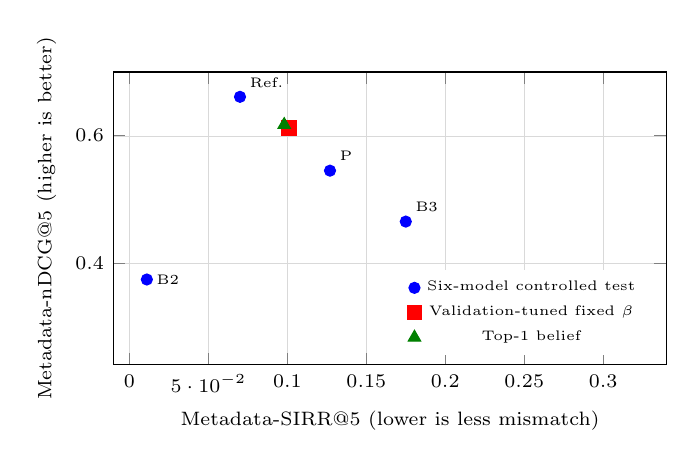
\begin{tikzpicture}
\begin{axis}[
  width=8.6cm, height=5.3cm,
  xlabel={Metadata-SIRR@5 (lower is less mismatch)},
  ylabel={Metadata-nDCG@5 (higher is better)},
  xmin=-0.01, xmax=0.34, ymin=0.24, ymax=0.70,
  tick label style={font=\scriptsize},
  label style={font=\scriptsize},
  grid=major, grid style={line width=0.1pt, draw=black!15},
  legend style={at={(0.97,0.03)},anchor=south east,font=\tiny,draw=none},
]
\addplot[only marks,mark=*,mark size=2pt,blue] coordinates {
(0.218,0.283) (0.301,0.343) (0.011,0.374) (0.175,0.465)
(0.127,0.545) (0.070,0.661)};
\addlegendentry{Six-model controlled test}
\addplot[only marks,mark=square*,mark size=2.6pt,red] coordinates {(0.101,0.612)};
\addlegendentry{Validation-tuned fixed $\beta$}
\addplot[only marks,mark=triangle*,mark size=2.6pt,green!50!black] coordinates {(0.098,0.617)};
\addlegendentry{Top-1 belief}
\node[font=\tiny,anchor=south west] at (axis cs:0.218,0.283) {B0};
\node[font=\tiny,anchor=south east] at (axis cs:0.301,0.343) {B1};
\node[font=\tiny,anchor=west] at (axis cs:0.011,0.374) {B2};
\node[font=\tiny,anchor=south west] at (axis cs:0.175,0.465) {B3};
\node[font=\tiny,anchor=south west] at (axis cs:0.127,0.545) {P};
\node[font=\tiny,anchor=south west] at (axis cs:0.070,0.661) {Ref.};
\end{axis}
\end{tikzpicture}
}
\caption{Ranking versus \emph{metadata-defined stage mismatch}, not independent agronomic safety. The validation-tuned and top-1 variants are shown separately from untuned B3.}
\label{fig:tradeoff}
\end{figure}

\section{Discussion}

\textbf{RQ1.} The historical three-seed ResNet-18 test accuracy is about 0.800 against six morphology-derived pseudo-stages, exceeding the majority reference (0.335). Since training seeds share one split and only 24 reproductive and ten grain-filling test crops, repeatability on the fixed subset is not independent field replication. Calibration and selective-risk results are evaluated against these weak labels.

\textbf{RQ2.} In the corrected English-language retrieval setting, adaptive gating improves metadata-defined ranking and mismatch over B1. Hard filtering has the lowest mismatch but sacrifices complete Top-5 coverage. Validation-tuned fixed-soft and top-1 belief outperform the original combined-confidence adaptive approach; the paper therefore evaluates a trade-off, \emph{not} universal superiority of adaptivity.

\textbf{RQ3.} The 420 scenarios are conditional on topic-stage eligibility (199 of 263 test crops) and nested within 63 parent photographs. Retrieval relevance and SIRR are derived from the same stage-compatibility annotations consumed by reranking. Consequently, these are controlled mechanism-consistency scores, not independent recommendation-quality or field-safety measurements.

\section{Limitations and Ethical Considerations}
\label{sec:limitations}

The labels are deterministic, BBCH-inspired pseudo-stages, not agronomist-confirmed phenological observations. One ResNet-18 backbone and one fixed split cannot establish generalization across fields, seasons, cultivars or acquisition devices. Rare-stage support is limited, and grouping by aHash reduces detected duplication without demonstrating new-field independence. Retrieval's metadata-derived judgments may favor algorithms using that metadata; no independent expert relevance or agronomic-safety reference is available. These are intrinsic evidence boundaries, not uncompleted experiments.

\textit{Ethical considerations.} Crop photographs may expose location or personal details; publish source images only under the relevant permissions and remove identifying metadata absent consent. The system is not an autonomous agronomic decision authority: regulated or high-impact recommendations require qualified human judgment.

\section{Conclusion}

CropState-Vision evaluates six weakly supervised rice pseudo-stages and stage-aware retrieval with explicit uncertainty and provenance controls. ResNet-18 accuracy is approximately 0.800 on a fixed split. On 420 scenarios, Adaptive improves metadata nDCG@5 from 0.343 to 0.545 over query expansion and lowers metadata-SIRR@5 from 0.301 to 0.127. However, validation-tuned fixed-soft reaches 0.612/0.101 and top-1 belief reaches 0.617/0.098, exceeding combined-confidence Adaptive on these metadata measures. Hard filtering minimizes mismatch at the cost of underfilled Top-5 outputs. These results support an internal evaluation framework, not a claim of expert-confirmed BBCH accuracy, agronomic usefulness or field safety.

\textit{Data and code availability.} The 2{,}900-crop benchmark is derived from RiceSEG \cite{zhou2025riceseg}; the 173 English chunks are machine-curated from IRRI public knowledge material \cite{irri_knowledge_bank}. Underlying photos and source text retain their original access conditions. Reproduction code and permitted configuration/provenance records are at \texttt{github.com/khov4nfs/cropstate}.

\bibliographystyle{IEEEtran}
\bibliography{references}

\end{document}
